\documentclass[pdf]{beamer}
\mode<presentation>{}
\usetheme{Dresden}
\usepackage{apalike}
\usepackage{graphicx}
\usepackage{subcaption}
\usepackage{pgfplotstable}
\usepackage{graphicx,psfrag}
\usepackage{amssymb}
\usepackage{mwe,tikz}\usepackage[percent]{overpic}
\usepackage{pifont}% http://ctan.org/pkg/pifont
\newcommand{\cmark}{\ding{51}}%
\newcommand{\xmark}{\ding{55}}%

%% preamble
\title{Dispersive Shock Waves of the Serre equations}
\author{Jordan Pitt, Stephen Roberts and Christopher Zoppou \\ Australian National University}
\newcommand\solidrule[1][0.25cm]{\rule[0.5ex]{#1}{1pt}}
\newcommand\dashedrule{\mbox{\solidrule[2mm]\hspace{2mm}\solidrule[2mm]}}
\newcommand{\dotrule}[1]{%
	\parbox[]{#1}{\dotfill}}

\begin{document}
%% title frame
\section{Introduction}
\begin{frame}
\titlepage
\end{frame}
\subsection{Introduction}

\begin{frame}{Outline of the Presentation}
	\begin{itemize}
		\item Motivation
		\item Serre Equations
		\item Dispersive Shock Waves
		\item Numerical Experiment
		\item Results
	\end{itemize}
\end{frame}

\begin{frame}<1>[label=BG]{Our Background}
	\begin{tabular}{l l l l}
		{ \color[RGB]{59,50,164} \usebeamertemplate{itemize item}{} } &Interest &:& Numerical methods for water waves. \\ &&&Focusing on ocean hazards. \\ \\
		\pause
		{ \color[RGB]{59,50,164} \usebeamertemplate{itemize item}{} } &Resulted In &:& Robust numerical method for the \\ &&& Shallow Water Wave Equations (ANUGA) \\\\
		\pause
		{ \color[RGB]{59,50,164} \usebeamertemplate{itemize item}{} } & Current Goal &:& Robust numerical method for the \\ &&& Serre equations\\\\
		\pause
		{ \color[RGB]{59,50,164} \usebeamertemplate{itemize item}{} } &Problem &:& Evolution of shocks for the Serre equations
	\end{tabular}
\end{frame}

\begin{frame}{Indian ocean tsunami}
	\begin{figure}
		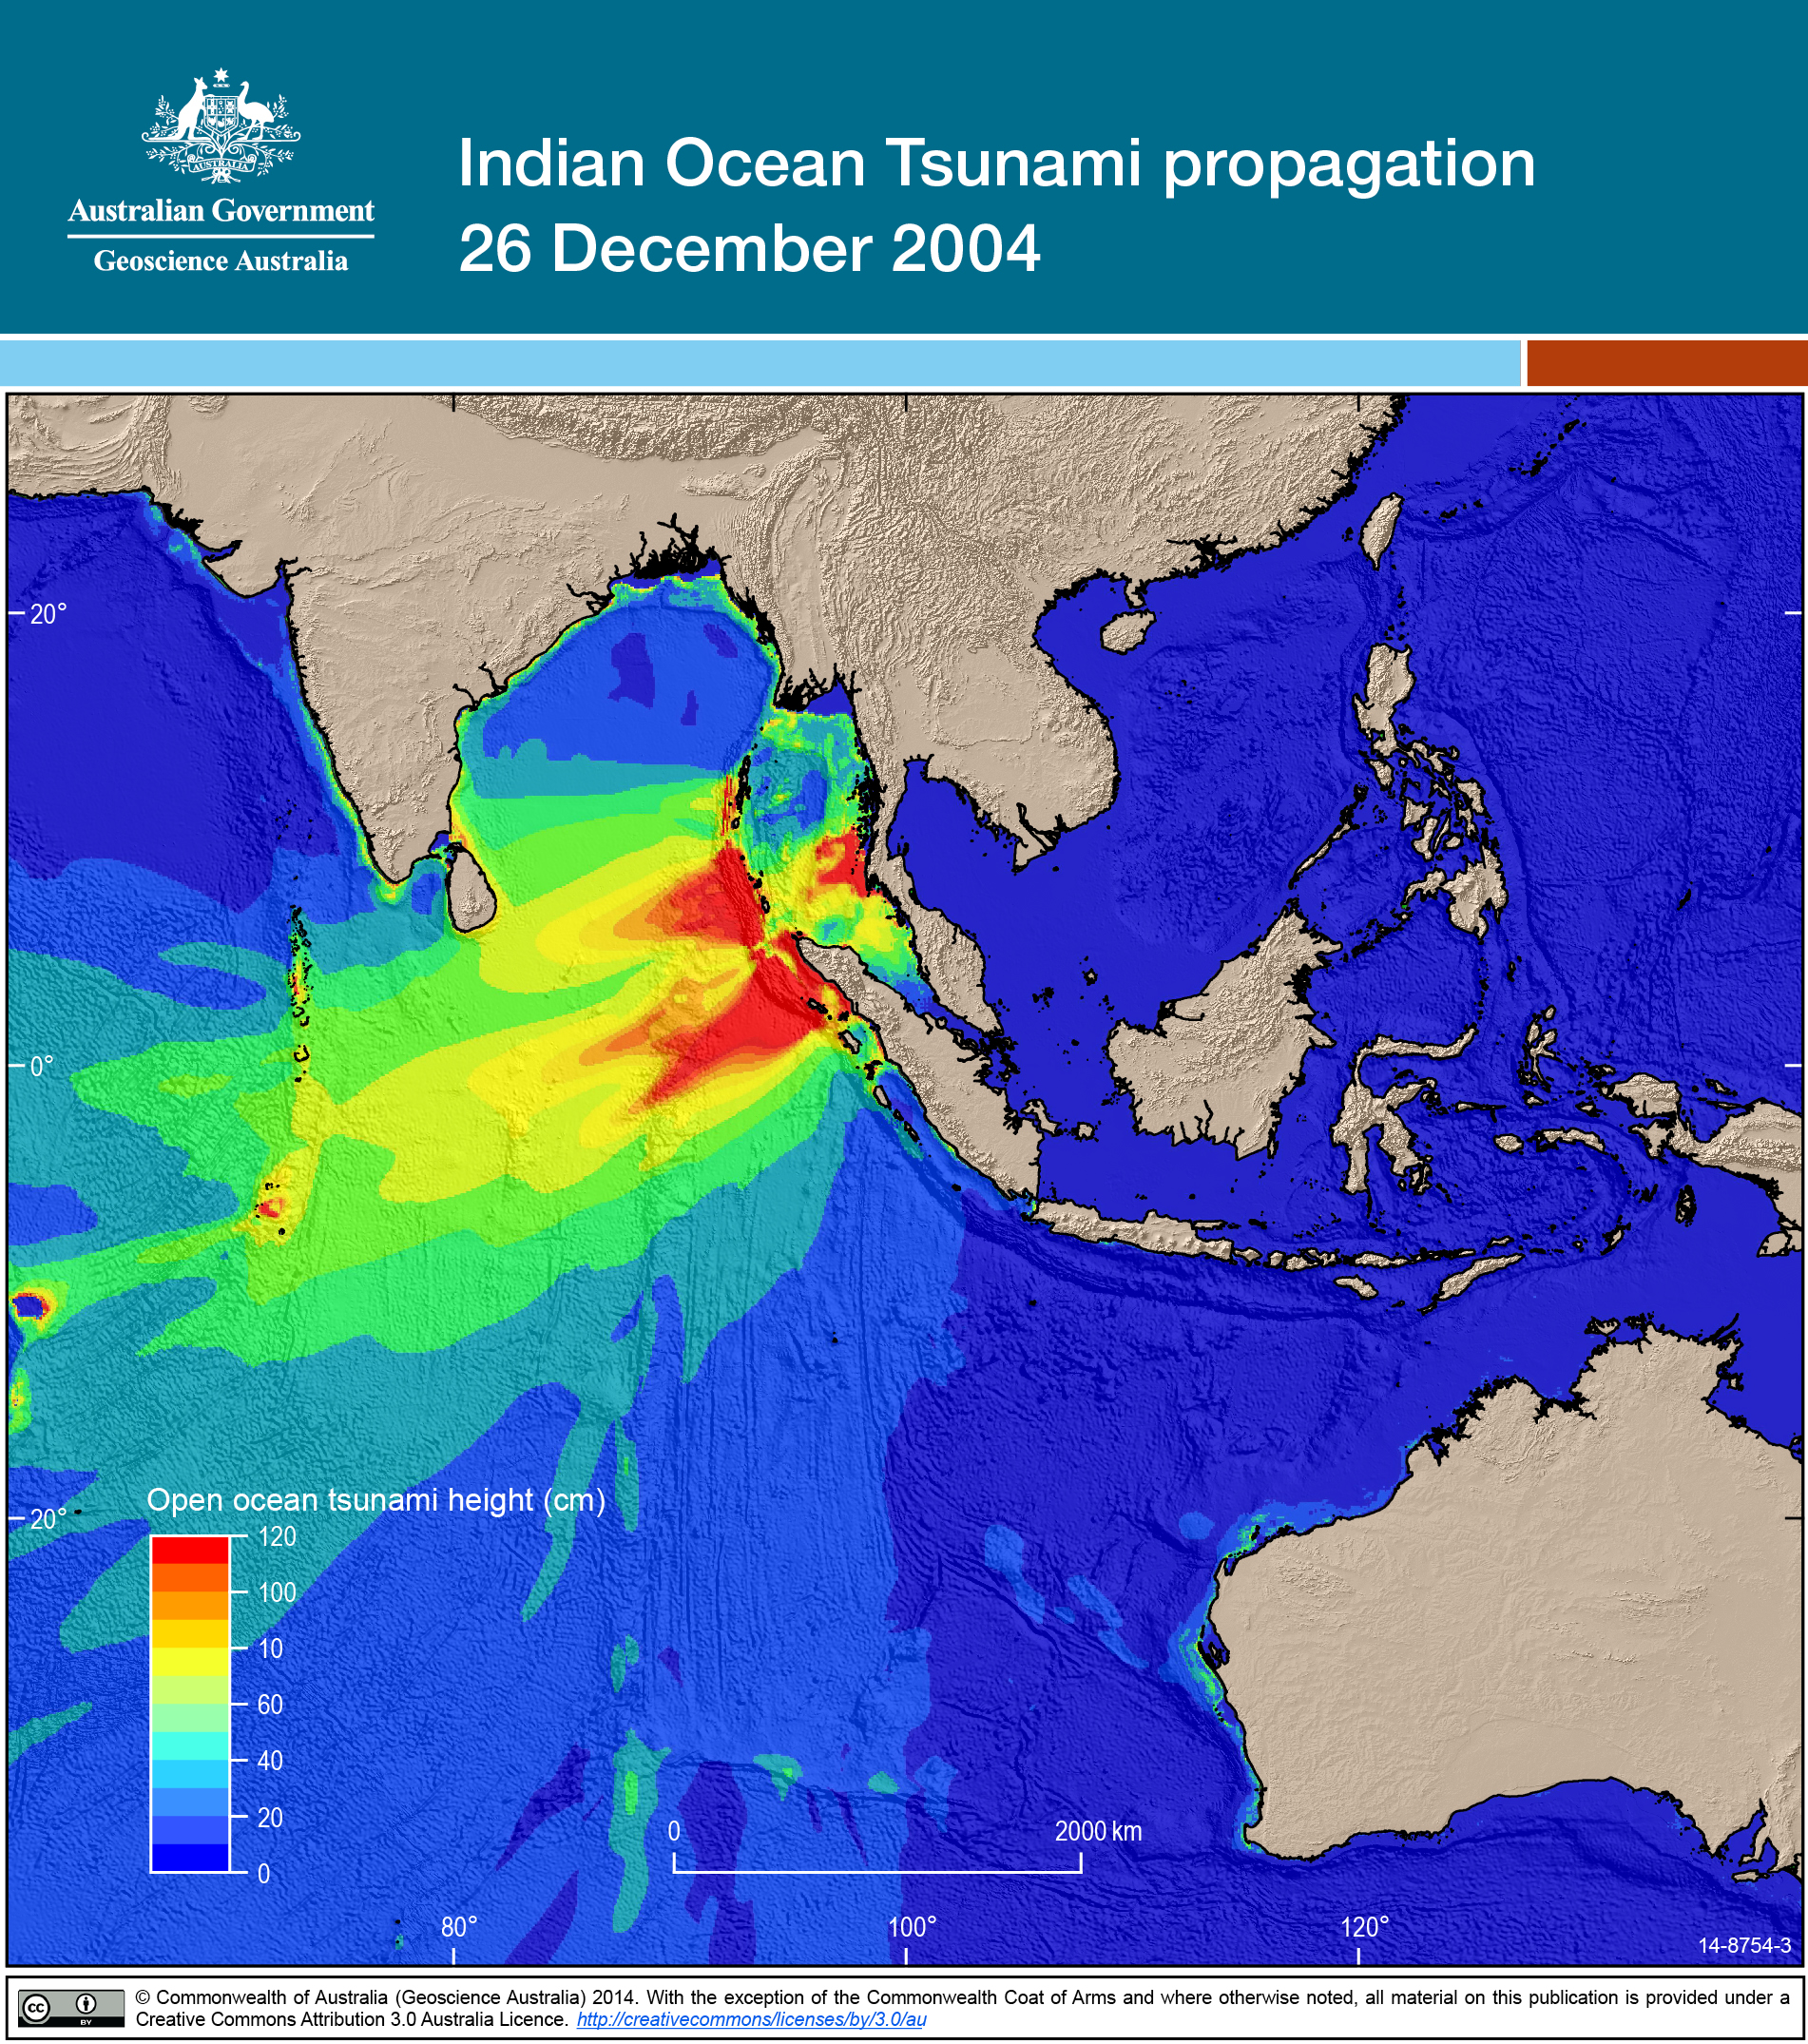
\includegraphics[width=5cm]{./Pictures/Introduction/IOT.jpg}
	\end{figure}
\end{frame}

\againframe<2>{BG}


\begin{frame}{Depth Averaged Equations}
	\begin{figure}
		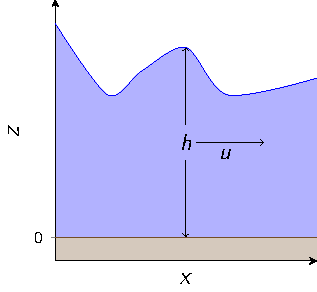
\includegraphics[width=6cm]{./Pictures/Drawn/DepthAveraged.pdf}
	\end{figure}
\end{frame}

\begin{frame}{Shallow Water Wave Equations}
	Conservation of Mass
	\[
	\dfrac{\partial h}{\partial t} + \dfrac{\partial (uh)}{\partial x} = 0
	\]
	
	Conservation of Momentum
	\begin{equation*}
	\dfrac{\partial (uh)}{\partial t} + \dfrac{\partial}{\partial x} \left ( u^2h + \dfrac{gh^2}{2}   \right )  = 0
	\end{equation*}
\end{frame}

\againframe<3>{BG}

\begin{frame}{Serre equations}
	
	Conservation of Mass
	\[
	\dfrac{\partial h}{\partial t} + \dfrac{\partial (uh)}{\partial x} = 0
	\]
	
	Conservation of Momentum
	\begin{equation*}
	 \dfrac{\partial (uh)}{\partial t} + \dfrac{\partial}{\partial x} \left ( u^2h + \dfrac{gh^2}{2} + \dfrac{h^3}{3}{\color{red} \Phi }   \right )  = 0
	\end{equation*}
	
	\[ 	{\color{red} \Phi }  = \dfrac{\partial u }{\partial x} \dfrac{\partial u}{\partial x} -u \dfrac{\partial^2 u}{\partial x^2}  - \dfrac{\partial^2 u}{\partial x \partial t}  \]
\end{frame}

\againframe<4>{BG}


\section{Dispersive Shock Waves}
\subsection{Introduction}
\begin{frame}{Dispersive Shock Waves}
		
   \begin{figure}
    	\centering
    	\begin{minipage}{.5\textwidth}
    		\centering
    		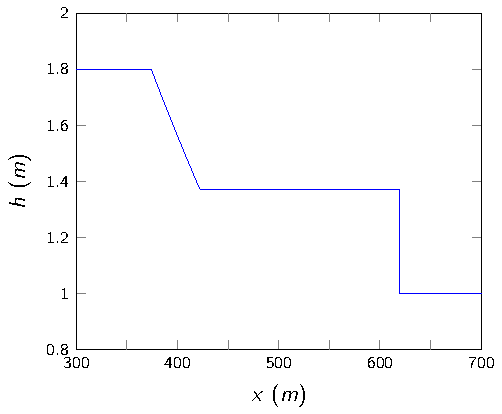
\includegraphics[width=0.9\linewidth]{./Pictures/DSW/SW.pdf}
    		\caption{Shock Wave (analytical solution of the shallow water wave equations).}
    	\end{minipage}%
    	\begin{minipage}{.5\textwidth}
    		\centering
    		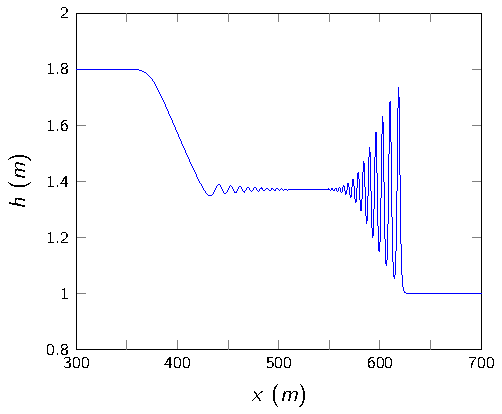
\includegraphics[width=0.9\linewidth]{./Pictures/DSW/DSW.pdf}
    		\caption{Dispersive Shock Wave (numerical solution of the Serre equations).}
    	\end{minipage}
   \end{figure}
\end{frame}

\begin{frame}<1>[label=test]{Properties of DSW for the Serre Equations}
	Asymptotic results for long times
	\begin{itemize}
		\item Whitham modulation results for leading wave amplitude and speed \pause
		\item Oscillations of the DSW for the Serre equations oscillate around the SW of the SWWE \newline 
		\pause
	\end{itemize}
	Linear results
		\begin{itemize}
			\item Separate dispersive tails
		\end{itemize}
\end{frame}

\begin{frame}{Whitham Modulation Results}
	\begin{figure}
		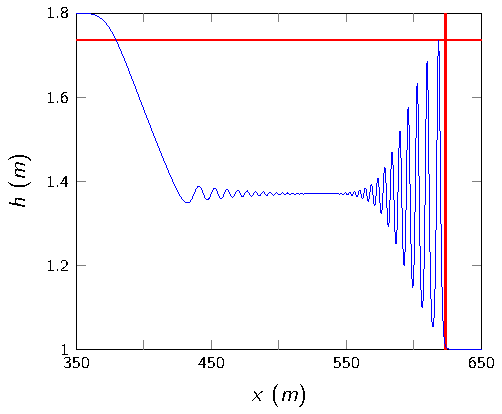
\includegraphics[width=0.7\textwidth]{./Pictures/DSW/DSWap.pdf}
	\end{figure}
\end{frame}

\againframe<2>{test}

\begin{frame}{DSW comparison to SW}
	\begin{figure}
		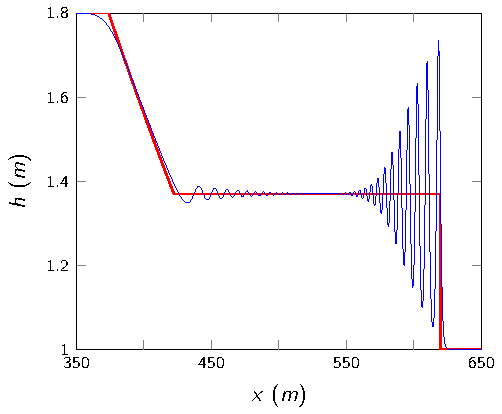
\includegraphics[width=0.7\textwidth]{./Pictures/DSW/DSWcompSW.pdf}
	\end{figure}
\end{frame}

\againframe<3>{test}

\begin{frame}{Separation of Dispersive Tails}
	\begin{figure}
		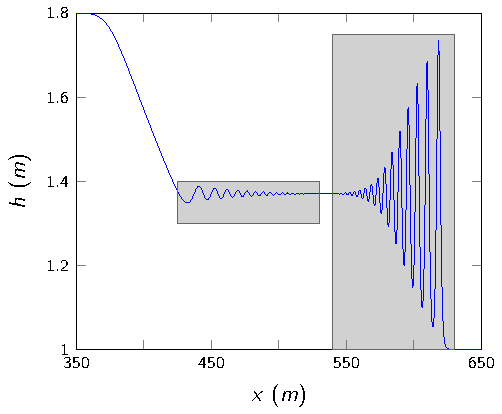
\includegraphics[width=0.7\textwidth]{./Pictures/DSW/DSWtails.pdf}
	\end{figure}
\end{frame}

\begin{frame}{Problem}
	No analytic solution of the Serre equations for DSW
\end{frame}

\subsection{Numerical Solutions}
\begin{frame}{Numerical Solutions}
	\begin{itemize}
		\item Few numerical solutions in the literature for DSW
		\item Most common numerical solutions are for the dam-break problem or a smooth approximation to it
	\end{itemize}
\end{frame}

\begin{frame}{Model Problem : Dam Break Problem}
	\begin{subequations}
		\begin{gather*}
		h(x,0) = \left\lbrace \begin{array}{c c}
		h_1  & x \le x_0\\ h_0  & x > x_0 
		\end{array} \right. 
		\end{gather*}
		\begin{gather*}
		u(x,0) = 0.0 .
		\end{gather*}
	\end{subequations} 

\end{frame}

\begin{frame}{Dam Break Problem Example}

$h_0 = 1m$, $h_1 = 1.8m$ and $x_0 = 500m$
	\begin{figure}
		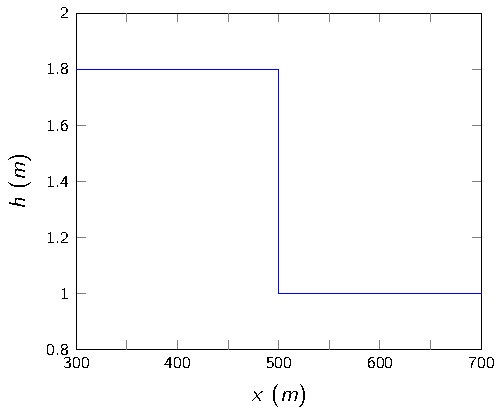
\includegraphics[width=0.7\textwidth]{./Pictures/DSW/DBinit.pdf}
	\end{figure}

\end{frame}

\begin{frame}{Smoothed Approximation : Smoothed Dam Break Problem}
	\begin{subequations}
		\begin{gather*}
		h(x,0) = h_0  + \frac{h_1 - h_0}{2} \left(1 + \text{tanh}\left(\frac{x_0 - x}{\alpha}\right)\right) 
		\end{gather*}
		\begin{gather*}
		u(x,0) = 0.0 .
		\end{gather*}
	\end{subequations} 
	
\end{frame}

\begin{frame}{Smoothed Dam Break Problem Example}
	
	$h_0 = 1m$, $h_1 = 1.8m$ and $x_0 = 500m$
	\begin{figure}
		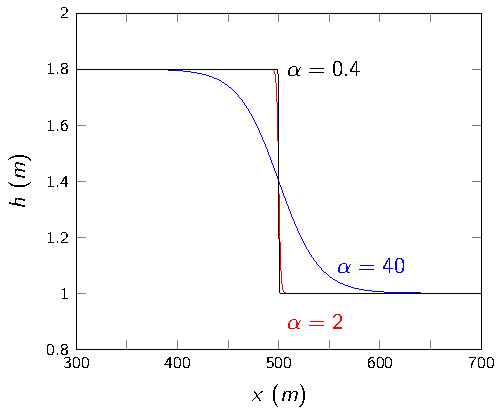
\includegraphics[width=0.7\textwidth]{./Pictures/DSW/DBSinit.pdf}
	\end{figure}
	
\end{frame}

%smoothed


\begin{frame}{Grimshaw's Results (2006)}
	\begin{figure}
		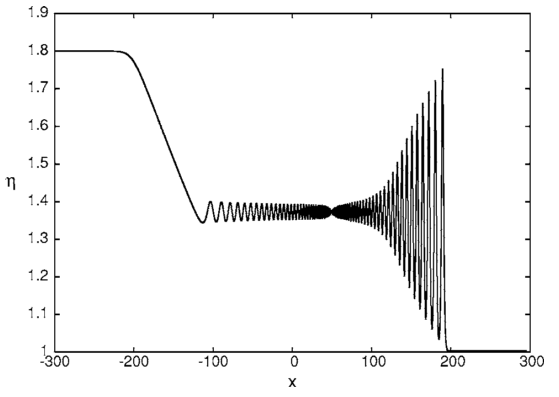
\includegraphics[width=0.6\textwidth]{./Pictures/DSW/SmoothDBEl.png}
	\end{figure}
	Numerical solution of second-order finite difference method for a smooth approximation to the dam break problem
\end{frame}

\begin{frame}{Hanks Results (2010)}
	\begin{figure}
		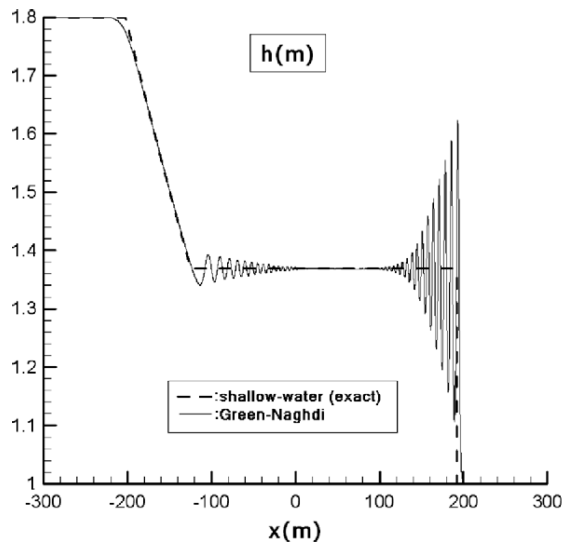
\includegraphics[width=0.45\textwidth]{./Pictures/DSW/DBhankcut.png}
	\end{figure}
	Numerical solution of first-order hybrid finite difference volume method for dam break problem
\end{frame}

\begin{frame}{Mitsotakis Results (2014)}
	\begin{figure}
		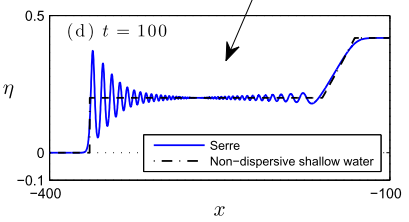
\includegraphics[width=0.8\textwidth]{./Pictures/DSW/SmoothDBDutyhkcut.png}
	\end{figure}
	Numerical solution of fourth-order finite element method for smoothed dam break problem ($\alpha = 1$)
\end{frame}

\begin{frame}{Problem}
	Numerical results in the literature have different behaviours, although most publications report the completely separated dispersive tails of Hank and Mitsotakis[]
	
	Questions:
	\begin{itemize}
		\item Which behaviour is correct?
		\item What is the effect of the numerical method?
		\item What is the effect of the smoothing of the dam-break problem?
	\end{itemize}
\end{frame}

\section{Experiment}
\subsection{Aim}
\begin{frame}{Aim}
	Investigate numerical solutions of the Serre equations to the smoothed dam-break problem with various
	\begin{itemize}
		\item values of $\alpha$
		\item numerical methods
	\end{itemize}
\end{frame}

\begin{frame}{Methods}
	Finite Difference Methods
	\begin{itemize}
		\item Naive second-order centered finte difference
		\item Finite difference of Grimshaw[]
	\end{itemize}
	Hybrid Finite Difference Volume Methods
	\begin{itemize}
		\item First-order (same method as Hank[])
		\item Second-order 
		\item Third-order 
	\end{itemize}
\end{frame}

\section{Results}
\begin{frame}{Observed Behaviours}
	We observed and justified four different behaviours of the numerical solution for the DSW \newline \newline
	Main cause of the different behaviours was the $\alpha$ value \newline \newline
	We demonstrate the different observed behaviours here using the third-order hybrid method's highest resolution numerical solution for a particular $\alpha$ value
\end{frame}

\begin{frame}{Non Oscillatory Structure $\alpha = 40$}
	\begin{figure}
		\includegraphics[width=0.65\textwidth]{./Pictures/Results/Example/noni.pdf}
		\caption{Initial conditions}
	\end{figure}
\end{frame}

\begin{frame}{Non Oscillatory Structure $\alpha = 40$}
		\begin{figure}
			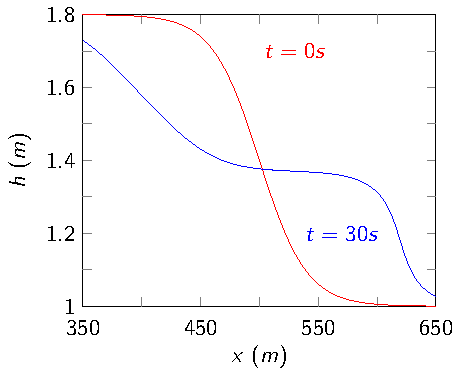
\includegraphics[width=0.65\textwidth]{./Pictures/Results/Example/non.pdf}
			\caption{Highest resolution third-order numerical solution at $t=30s$}
		\end{figure}
\end{frame}

\begin{frame}{Flat Structure $\alpha = 2$}
	\begin{figure}
		\includegraphics[width=0.65\textwidth]{./Pictures/Results/Example/flati.pdf}
		\caption{Initial conditions}
	\end{figure}
\end{frame}

\begin{frame}{Flat Structure $\alpha = 2$}
	\begin{figure}
		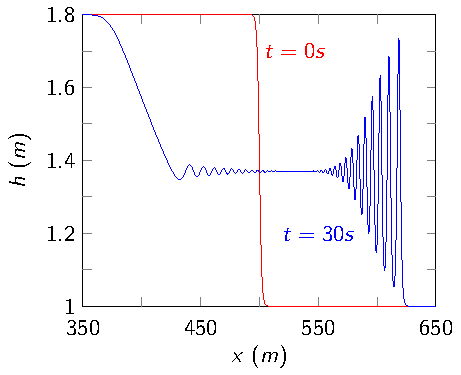
\includegraphics[width=0.65\textwidth]{./Pictures/Results/Example/flate.pdf}
		\caption{Highest resolution third-order numerical solution at $t=30s$}
	\end{figure}
\end{frame}

\begin{frame}{Node Structure $\alpha = 0.4$}
	\begin{figure}
		\includegraphics[width=0.65\textwidth]{./Pictures/Results/Example/nodei.pdf}
		\caption{Initial conditions}
	\end{figure}
\end{frame}

\begin{frame}{Node Structure $\alpha = 0.4$}
	\begin{figure}
		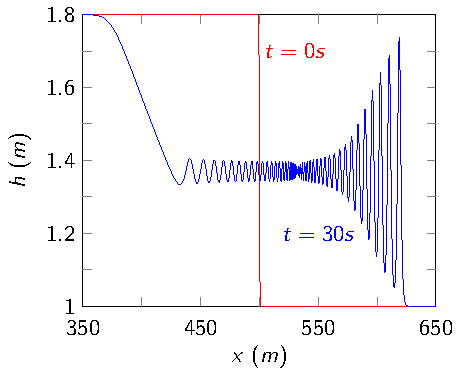
\includegraphics[width=0.65\textwidth]{./Pictures/Results/Example/node.pdf}
		\caption{Highest resolution third-order numerical solution at $t=30s$}
	\end{figure}
\end{frame}

\begin{frame}{Growth Structure $\alpha = 0.1$}
	\begin{figure}
		\includegraphics[width=0.65\textwidth]{./Pictures/Results/Example/growthi.pdf}
		\caption{Initial conditions}
	\end{figure}
\end{frame}

\begin{frame}{Growth Structure $\alpha = 0.1$}
	\begin{figure}
		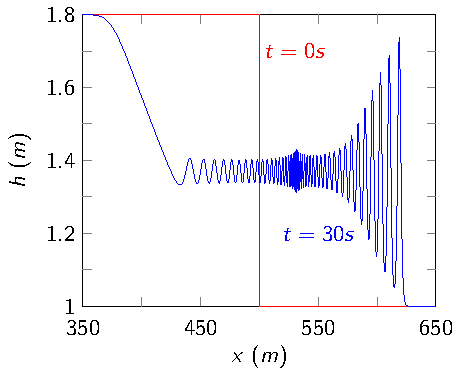
\includegraphics[width=0.65\textwidth]{./Pictures/Results/Example/growth.pdf}
		\caption{Highest resolution third-order numerical solution at $t=30s$}
	\end{figure}
\end{frame}

\begin{frame}{Justifying These Numerical Solutions}
	For a particular numerical method and $\alpha$ value:
	\begin{itemize}
		\item Demonstrated convergence as the resolution of the method increases
		\item Demonstrated numerical solutions conserve mass, momentum and the Hamiltonian
	\end{itemize}
\end{frame}

\begin{frame}{Answers}
	Questions:
	\begin{itemize}
		\item Which behaviour is correct?
		\item What is the effect of the numerical method?
		\item What is the effect of the smoothing of the dam-break problem?
	\end{itemize}
\end{frame}

\begin{frame}{Which behaviour is correct?}
	\begin{itemize}
		\item Depends on the $\alpha$ value.
		\item These results demonstrate that for solving the dam-break problem we expect the growth structure for short time periods.
		\item For longer time periods as time increases the growth structure decays to the node structure which then decays to the flat structure.
	\end{itemize}
\end{frame}

\begin{frame}{What is the effect of the numerical method?}
	\begin{itemize}
		\item Diffusive first-order methods limit the observable behaviours with reasonable resolutions. In particular we will not get the growth structure for the DSW of the dam-break problem unless we use very fine resolutions.
		\item All higher-order methods reproduce all the observed behaviours
		\item Hybrid finite difference volume methods more robust than the finite difference methods for small $\alpha$ values
	\end{itemize}
\end{frame}

\begin{frame}{What is the effect of the smoothing of the dam-break problem?}
	\begin{itemize}
		\item Most important factor determining the observed behaviour
		\item Observed behaviour sensitive to the smoothing of the problem
	\end{itemize}
\end{frame}


\begin{frame}{Properties of DSW for the Serre Equations}
	Asymptotic results [] (long time solutions)
	\begin{itemize}
		\item Whitham modulation results for leading wave amplitude and speed
		\item Oscillations of the DSW for the Serre equations oscillate around the SW of the SWWE \newline 
	\end{itemize}
	Linear results []
	\begin{itemize}
		\item Separate dispersive tails
	\end{itemize}
\end{frame}	

\begin{frame}{Properties of DSW for the Serre Equations}
	Asymptotic results [] (long time solutions)
	\begin{itemize}
		\item[{\color{green!60!black}\checkmark}] Whitham modulation results for leading wave amplitude and speed 
		\item Oscillations of the DSW for the Serre equations oscillate around the SW of the SWWE \newline 
	\end{itemize}
	Linear results []
	\begin{itemize}
		\item Separate dispersive tails
	\end{itemize}
\end{frame}	

\begin{frame}{Properties of DSW for the Serre Equations}
	Asymptotic results [] (long time solutions)
	\begin{itemize}
		\item[{\color{green!60!black}\checkmark}] Whitham modulation results for leading wave amplitude and speed 
		\item[{\color{green!60!black}\checkmark}] Oscillations of the DSW for the Serre equations oscillate around the SW of the SWWE \newline 
	\end{itemize}
	Linear results []
	\begin{itemize}
		\item  Separate dispersive tails
	\end{itemize}
\end{frame}

\begin{frame}{Properties of DSW for the Serre Equations}
	Asymptotic results [] (long time solutions)
	\begin{itemize}
		\item[{\color{green!60!black}\checkmark}] Whitham modulation results for leading wave amplitude and speed 
		\item[{\color{green!60!black}\checkmark}] Oscillations of the DSW for the Serre equations oscillate around the SW of the SWWE \newline 
	\end{itemize}
	Linear results []
	\begin{itemize}
		\item[{\color{red} \xmark}{ \color{black} /}{ \color{green!60!black}\checkmark}]  Separate dispersive tails
	\end{itemize}
\end{frame}

\begin{frame}{Conclusion}
	\begin{itemize}
		\item Explained the differences in behaviour for numerical solutions published in the literature
		\item Found new behaviour of DSW for short time spans not previously published in the literature
		\item Good agreement between numerical solutions and known properties of DSW for long time periods
		\item Justified the robustness of the hybrid finite difference volume methods
	\end{itemize}
\end{frame}





\end{document}